\nocite{pracbin}

\begin{markdown}

# Reverse Engineering Exercise 1: Basics

**[Binary Provided: `2010303027_hw_1_exercise_1.exe`]**

## Calculate the value that the instruction at `0x40301B` loads into the RDI register!

* `lea rdi, ds:400FFEh[rcx*8] ; RDI = 0x????????????????`
* *note: the value in my example differs slightly*

\noindent\s To answer this question we need to know the value of `rcx`. I've extracted the relevant instructions with IDA: see Code \ref{excerpt1.1}.
\s

\end{markdown}
\begin{lstlisting}[language={[x86masm]Assembler},name={excerpt of relevant instructions task 1.1},label={excerpt1.1}]
.text:0000000000403014                 mov     rcx, 0Ah
.text:000000000040301B                 lea     rdi, ds:400FFBh[rcx*8]
\end{lstlisting}
\begin{markdown}

The mov instruction (line 1) copies the value `Ah` (`10`) into `rcx`. With that out of the way we can calculate the value with Python:

`hex(0x400ffb + 8 * 0xa)` which return `0x40104b` to us.
\n
This means that after executing the instruction (at least for the first time) the calculated value would be: **`40104Bh`**.
\n
Let's test that in IDA. We set a break point (*F2*) at the `lea` instruction and step over it (*F8*). As we can see in Figure \ref{calc} it is indeed correct.
\begin{figure}[!htbp]
\centering
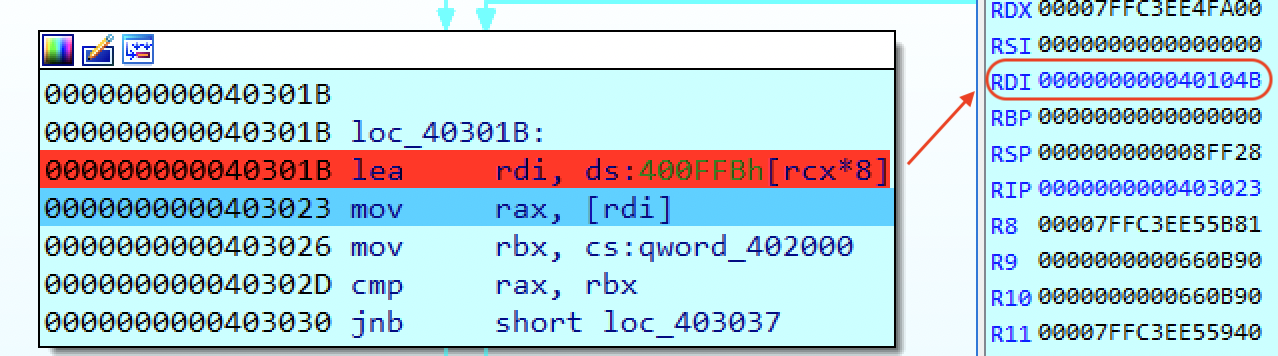
\includegraphics[width=.87\linewidth]{media/calc.png}
\caption{validating our calculation with IDA}\label{calc}
\end{figure}

## What is loaded into RAX when the instruction at address `0x403023` is run for the first time?

* `mov rax, qword[rdi] ; RAX = 0x????????????????`

\noindent\s
This builds on the previous example (the value of `rdi`). See Code \ref{excerpt1.2} for all relevant instructions.\s

\end{markdown}
\begin{lstlisting}[language={[x86masm]Assembler},name={excerpt of relevant instructions task 1.2},label={excerpt1.2}]
.text:0000000000403014           mov     rcx, 0Ah
.text:000000000040301B           lea     rdi, ds:400FFBh[rcx*8] ; rdi = 0x40104b
.text:0000000000403023           mov     rax, [rdi]
\end{lstlisting}
\begin{markdown}

The second `mov` instruction (line 3) copies the value that the address in `rdi` is pointing to into `rax`. Note the square brackets denoting dereferencing. Now all we need to know is where `0x40104b` points to.
\n
In IDA we can press *g* and jump to an address. We can either enter `0x40104b` or (if we're lazy and have stepped far enough) simply `rdi`. This leads us to to the data section (Code \ref{data1.2}).

\end{markdown}
\begin{lstlisting}[language={[x86masm]Assembler},name={excerpt of relevant data section task 1.2},label={data1.2}]
.data:000000000040104B db 0AFh
.data:000000000040104C db 0BEh
.data:000000000040104D db 0ADh
.data:000000000040104E db 0DEh
.data:000000000040104F db    0
.data:0000000000401050 db    0
.data:0000000000401051 db    0
.data:0000000000401052 db    0
\end{lstlisting}
\begin{markdown}

Reading it from the bottom up, our value is: **`DEADBEAFh`**, a classic.
\n
Same as before, let's make sure with IDA by stepping over it and taking a look at the register. Figure \ref{pred} shows us that we were correct.
\n
\begin{figure}[!htbp]
\centering
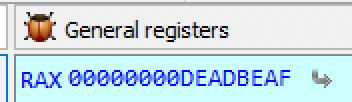
\includegraphics[width=.45\linewidth]{media/pred.png}
\caption{validating our prediction with IDA}\label{pred}
\end{figure}

\clearpage
## Is it possible that the application is defining an array of data somewhere in the program? If so what’s the address of the first element?

* Examine how the program access its data before you write the answer.

\noindent\s Let's get a rough overview of the program. IDAs graph view (*space*) is very useful for tasks like this. see Figure \ref{structure}, it starts right after the `scanf()` call and setting `rcx` to `10`.


\begin{figure}[!htbp]
\centering
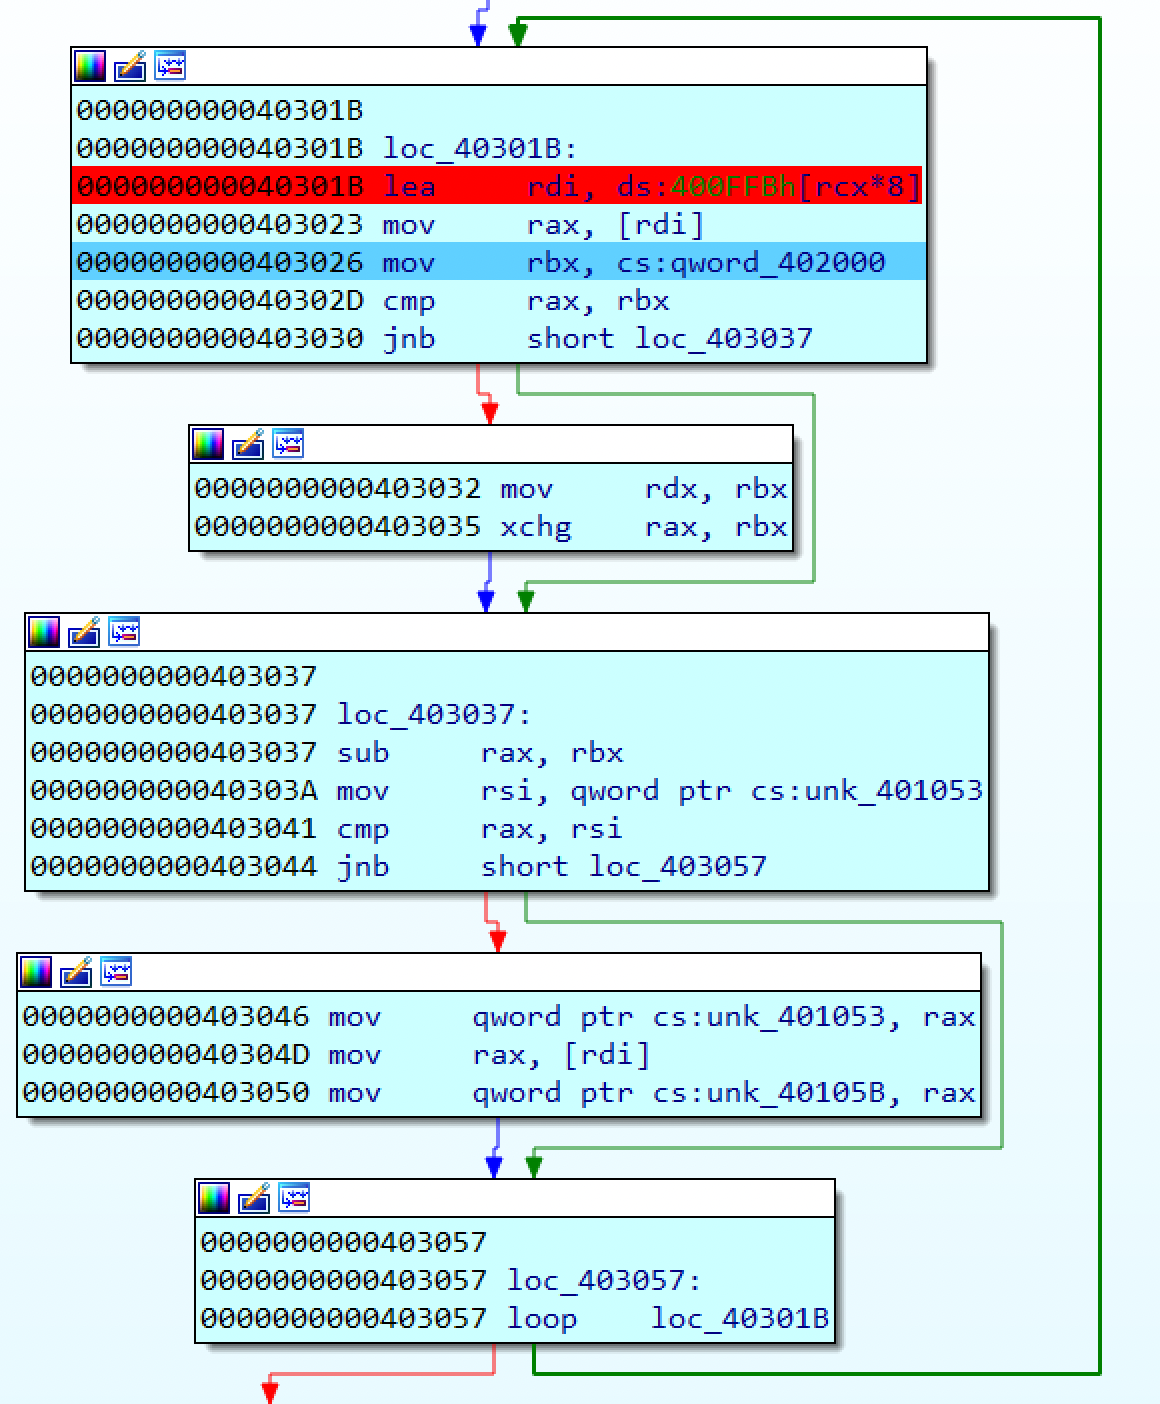
\includegraphics[width=.7\linewidth]{media/structure.png}
\caption{rough overview of the first program}\label{structure}
\end{figure}

\noindent The **first block** of code from `40301Bh` to `403030h` uses the value of the `rcx` register to calculate an address in the data section (notably in multiples of 8). As we have seen before the value of that address is subsequently loaded into the `rax` register.
\n
The **last block** of code (a single instruction) at `403057h` (conditionally) loops back to the first block. The `loop` instructions does the following:\s

* the counter register (`rcx`) is decremented by 1
* if the counter register is 0 the loop is terminated
* if not a jump is executed (in our case back to the first block) \cite{inteldev}

\noindent\s Let's take a look at the data section: jumping to `.data` puts us at the beginning of it, here we can find the format string.
\n
The array starts 4 byte after that (but is accessed in reverse order). After selecting the first element in IDA you can jump to the next element with *g* `+8` (and so forth).\s

\end{markdown}
\begin{lstlisting}[language={[x86masm]Assembler},name={beginning of array},label={data1.3}]
.data:0000000000401003 db '#',0 ; first element
.data:0000000000401005 db    0
.data:0000000000401006 db    0
.data:0000000000401007 db    0
.data:0000000000401008 db    0
.data:0000000000401009 db    0
.data:000000000040100A db    0
.data:000000000040100B db  75h ; second element
.data:000000000040100C db    0
.data:000000000040100D db    0
.data:000000000040100E db    0
; ...
\end{lstlisting}
\begin{markdown}

---

\noindent\s Here is how I came to that conclusion: the addresses (in the same order as accessed by the loop above) of all the elements of the array are the following -  via Python

`for rcx in range (10, 0, -1): print(hex(0x400ffb + rcx * 8))`

\begin{etaremune}
\item `0x40104b` (our `DEADBEAFh`)
\item `0x401043` (`433A34h`)
\item `0x40103b` (`2213h`)
\item `0x401033` (`5h`)
\item `0x40102b` (`100h`)
\item `0x401023` (`443h`)
\item `0x40101b` (`ABCh`)
\item `0x401013` (`111h`)
\item `0x40100b` (`75h`)
\item **`0x401003`** (`23h`)
\end{etaremune}

\noindent The counter variable starts at the bottom (`Ah` so `10` as a multiplier) and is subsequently decremented by 1. Since the loop is broken when `rcx` reaches zero the lowest `rcx` value to reach the instruction at `40301Bh` is `1`.
\n
The first element of the array is thus: `400FFBh + 1 * 8` which equals **`401003h`**. Each element has 8 Bytes (per the multiplier above).

## How many initialized global variables does this program define? 

Initialized global variables are located in the `.data` section. \cite{x64beg}. It starts at `0401000h` and ends at `402000h`.
\n
So far we have already encountered two:\s

* the format string starting at `401003h`
* the array starting at `401003h` (I'm going to count this as one)

\noindent\s They are joined by another two: quad-words at `401053h` and `40105Bh` (see Figure \ref{global})

\begin{figure}[!htbp]
\centering
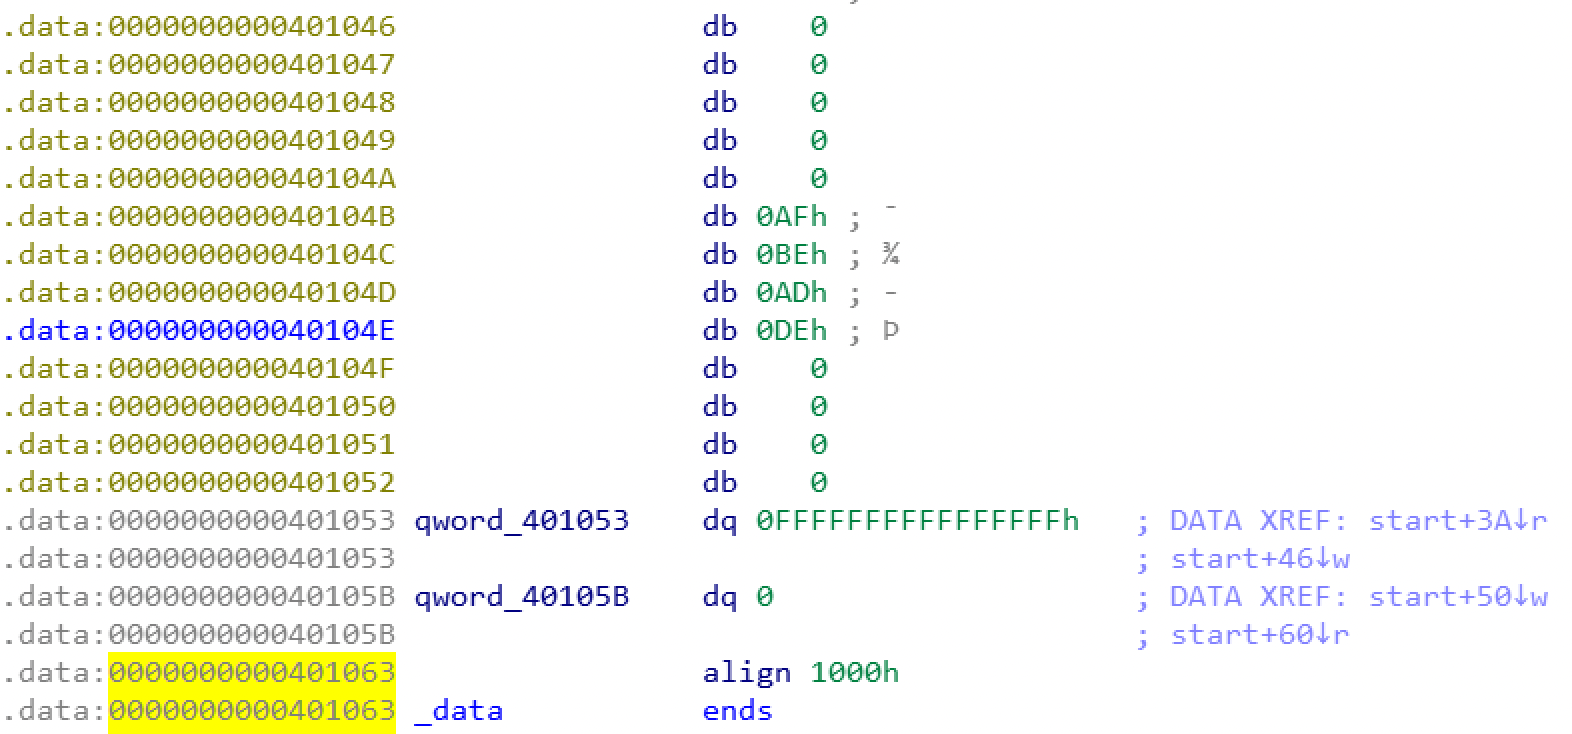
\includegraphics[width=1\linewidth]{media/global.png}
\caption{end of the array and the two quad-word (followed by no more discernible variables)}\label{global}
\end{figure}

\noindent The comment shows us where the two new quad-words are written and read from.

---

\noindent So **four** total.

## What happens if the value “433000” is passed to the program through the command line?

Passing the value `433000` to `2010303027_hw_1_exercise_1` results in the value `433A34` (see Figure \ref{433000}).

\begin{figure}[!htbp]
\centering
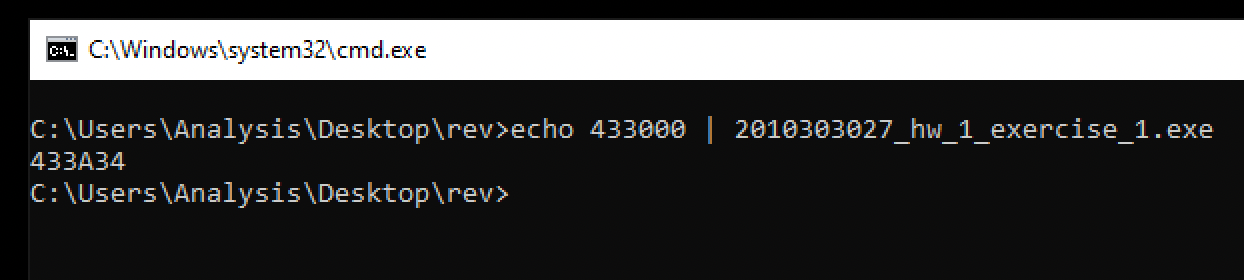
\includegraphics[width=\linewidth]{media/433000.png}
\caption{passing the value `433000` to `2010303027_hw_1_exercise_1.exe`}\label{433000}
\end{figure}

---

\noindent
I've also written a small Batch script that passes a range of values to possibly get a better understanding of the program without too much work: Code \ref{fuzzer}.
\newline
\end{markdown}
\begin{lstlisting}[language=command.com,name={fuzz.bat},label={fuzzer}]
@echo off
for /L %%G in (0, 1, 20000000) do (
  echo|set /p="%%G,  "
  echo %%G | C:\Users\ben\Desktop\2010303027\2010303027_hw_1_exercise_1.exe
  echo.
)
\end{lstlisting}
\begin{markdown}

Here is an excerpt of the output: Code \ref{log}.
\end{markdown}
\begin{lstlisting}[name={output via `fuzz.bat > log.txt`},label={log}]
0,  5
1,  5
# ...
13,  5
14,  5
15,  23
# ...
98,  75
99,  75
100,  111
101,  111
# ...
\end{lstlisting}
\begin{markdown}

It does give us a couple of input-value borders where the output value changes but is not particularly fast so I let it run in the background for a bit.
\n
Here is a list of values that I extracted from the log (on Linux via `sort -ut, -k2 log.txt`) before aborting the script. The left value is the first input value that results in a new output (right) value: \n

* 0,  5
* 15,  23
* 50,  75
* 100,  111
* 300,  443
* 780,  ABC
* 1000,  1000
* 1910,  2213
* 220000,  433A34

\noindent\s
Manually trying `-1` and random high values resulted in `DEADBEAF`, which are all (possibly) hex values. We already know all these values from our array!

\clearpage
## What does this program do? Describe it using your own words.

It reads input from the users and prints the closest value from an array.

---

\noindent Here's a more detailed outline (reference figure \ref{structure} for the loop):\s

* read **`user input`** as hexadecimal via `stdint` with `scanf()` (using format string `%X`)
* set **`counter`** register (`rcx`) to 10
* write **`user input`** to `402000h` in the `.bss` section (a quad-word)
* for each **`array element`** (from 10$^{th}$ to 1$^{st}$):
    * compare **`user input`** with **`array element`**:
        * if **`user input`** < **`array element`**: jump past switch
        * else: switch both values (simplifies the next step)
    * calculate absolute **`delta`**
    * compare **`delta`** with **`smallest known difference`** (that starts with max value):
        * if **`delta`** is lower update the **`smallest known difference`**
        * if **`delta`** is lower update the **`closest known element`**
    * decrement **`counter`**
* print the **`closest known element`** with `printf` (using the same format string)
* exit the program

\noindent\s The two quad-words we've seen in task 1.4 are used to store the `smallest known difference` (at `401053h`) and the `closest known element` (at `40105Bh`).

\clearpage
## Write a program that carries out the same task using any programming language you know
\end{markdown}
\begin{lstlisting}[language=python,name={finding the closest element with Python},label={python}]
#!/usr/bin/env python3

import sys


def get_closest_element():
    """
    this program prints the closest value from an array
    when compared with the userinput.
    """
    array = [
        0x23,
        0x75,
        0x111,
        0xABC,
        0x443,
        0x100,
        0x5,
        0x2213,
        0x433A34,
        0xDEADBEAF,
    ]

    user_input = int(input(), 16)
    smallest_difference = sys.maxsize
    closest_element = None

    # iterate through reversed array:
    for element in array[::-1]:
        # calculate current absolute delta.
        delta = abs(user_input - element)
        # update if we're closer:
        if delta < smallest_difference:
            smallest_difference = delta
            closest_element = element

    print(hex(closest_element))

if __name__ == "__main__":
    get_closest_element()
\end{lstlisting}
\begin{markdown}

\end{markdown}